\section{Data}
In this study, we use data products generated by the weekly intermittent Data Release Production (DRPs). 
These DRPs aim to test current data quality and produce LSST-like downstream data from the single-visit exposures. 
The week 49 DRP processed 4898 visits collected between 2025-04-17 and 2025-09-21 over an area of $\sim$ \SI{130}{\deg^2}. 
We only use visits labelled as "science" visits.
Figure~\ref{fig:footprint} shows the footprint of the data processed in the week 49 DRP 
This DRP processed visits from the COSMOS, M49, SV225\_40, ELAIS\_S1, ECDFS and EDFS A + B fields. 
It does not include the LSST SV1000 region.
\begin{figure}[h!]
    \centering
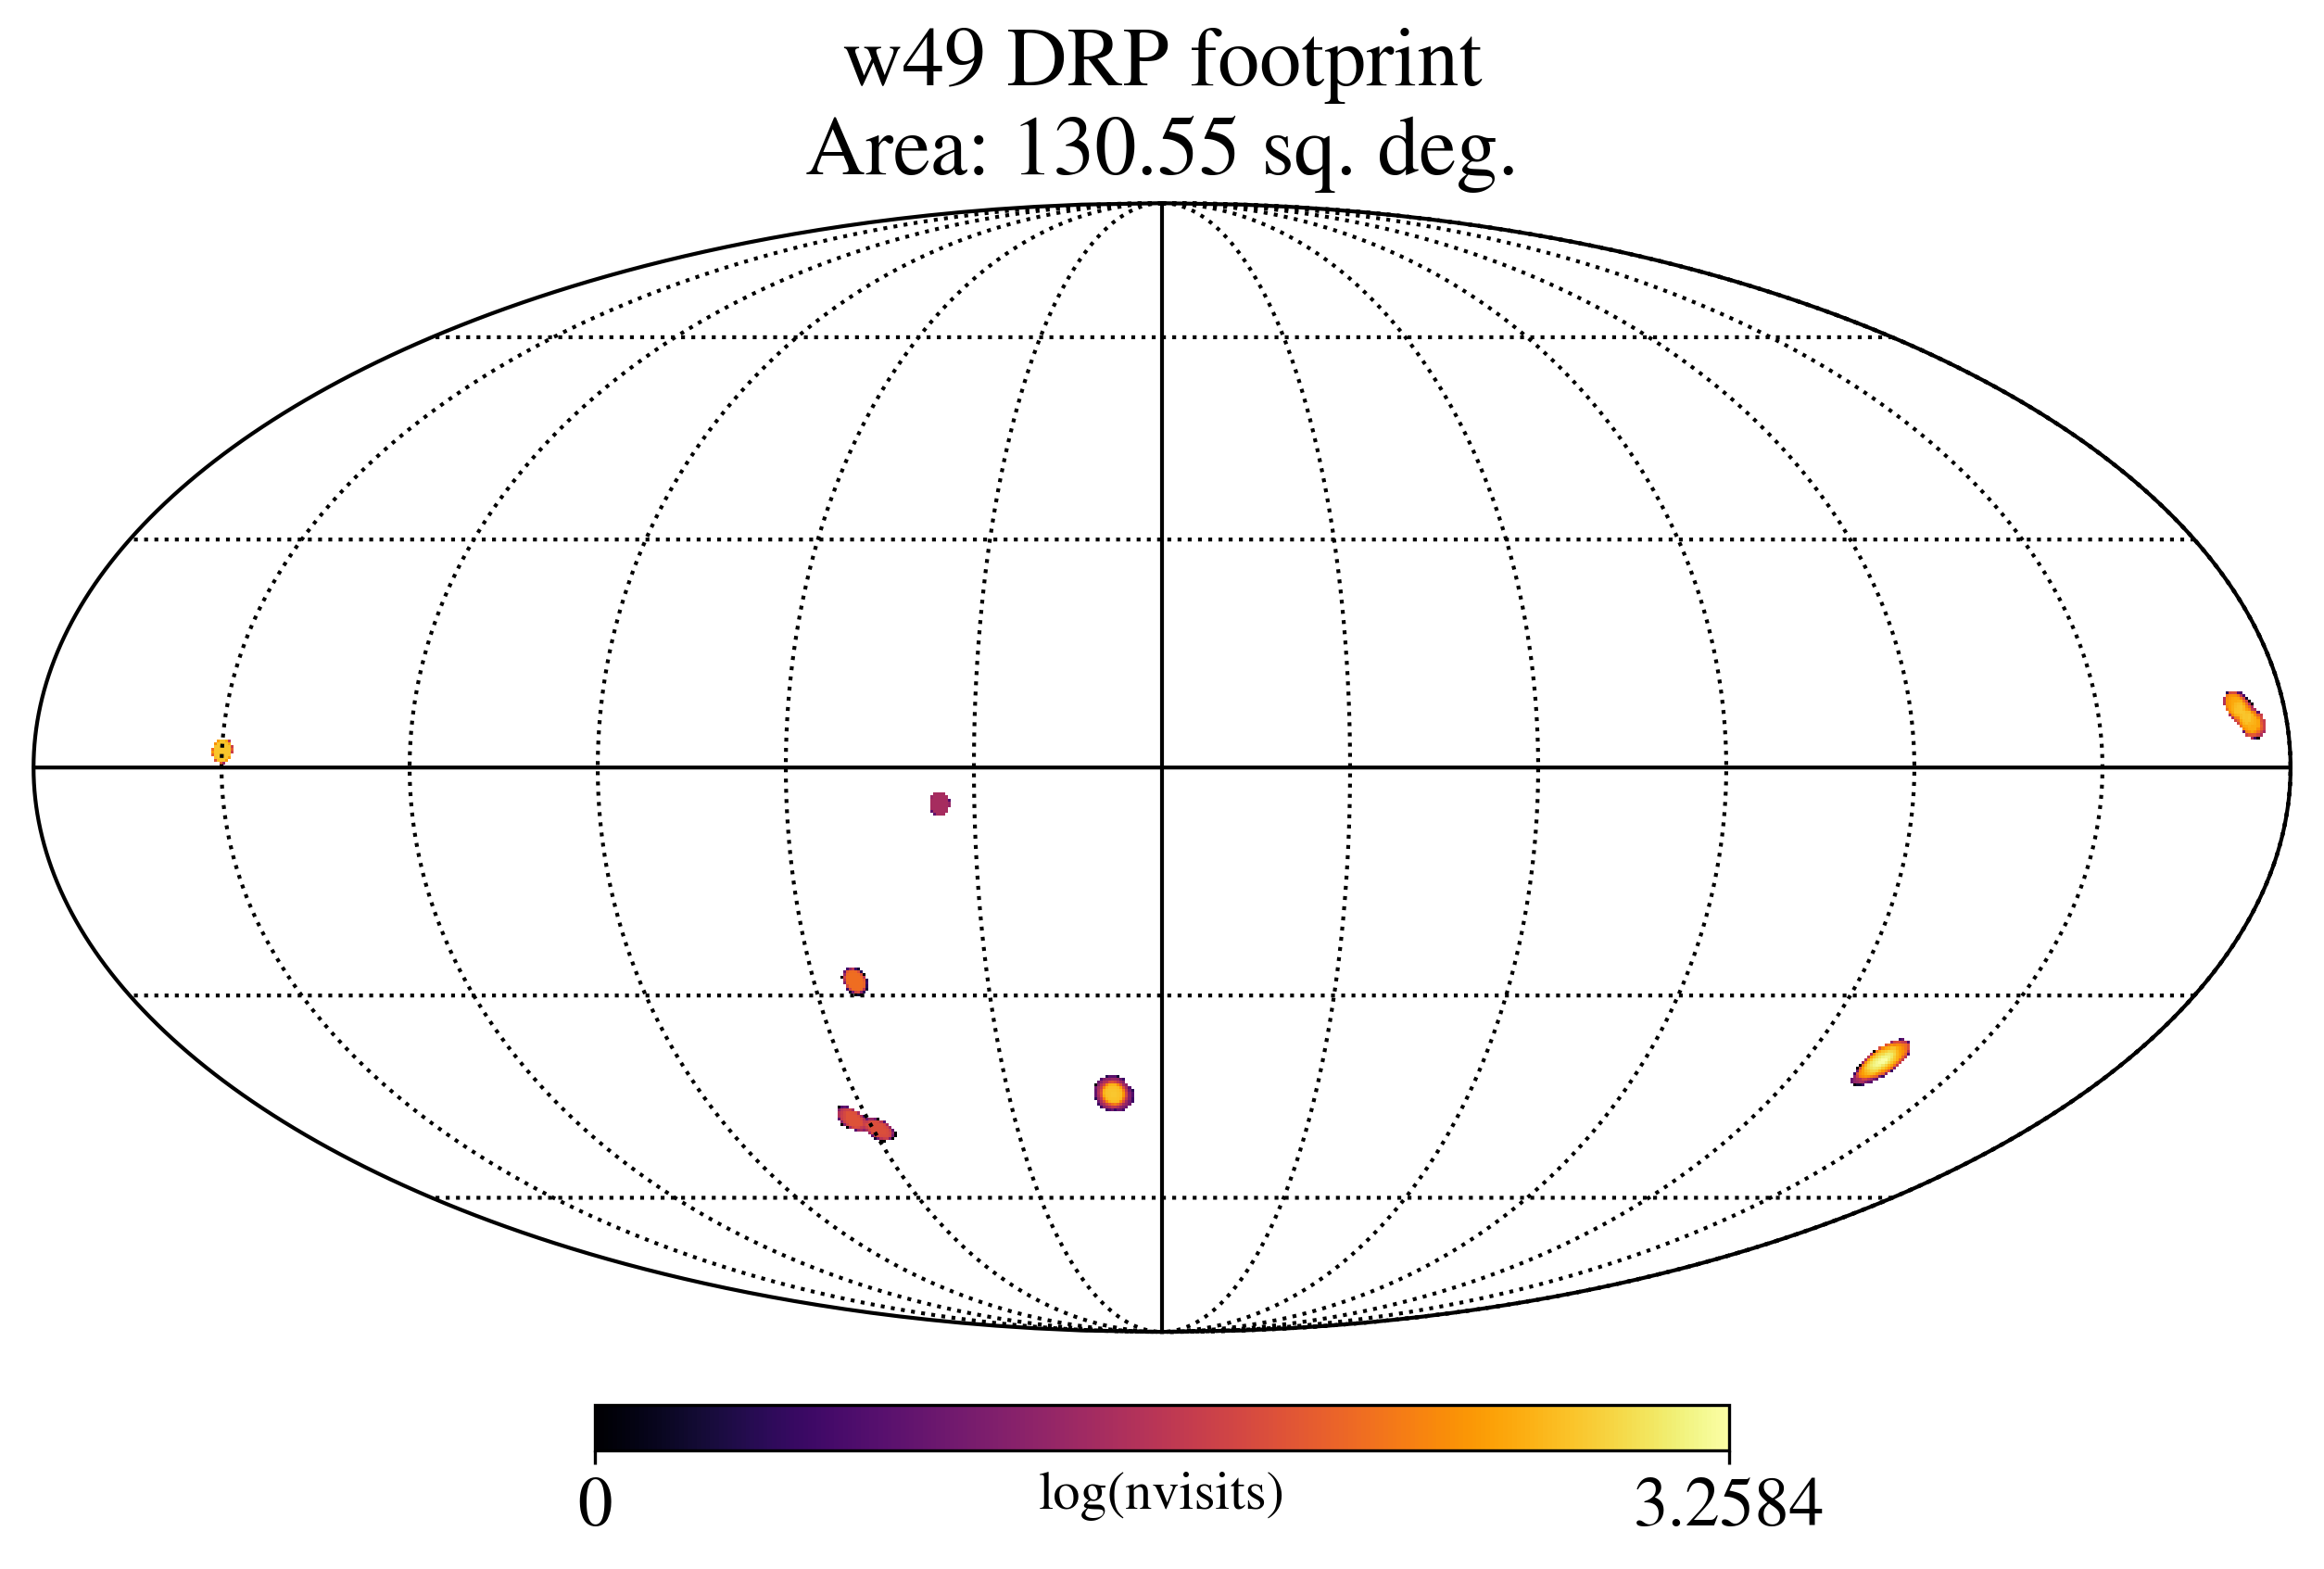
\includegraphics[width=0.8\textwidth]{figures/w49_footprint.png}
    \caption{week 49 DRP footprint, coloured by the number of visits collected in the pixel.} 
    \label{fig:footprint}
\end{figure}

We use two main data products: the \texttt{object} and the \texttt{refit\_psf\_star} tables.

The \texttt{object} table contains data of stars and galaxies derived from the per-band coadded images. 
The \texttt{refit\_psf\_star} table contains data of stars and galaxies derived from the single-visit images and PSF moments modelled with the \texttt{PiFF} package \citep{jarvis2021}.
For the purposes of this technote, we transform the moments from camera coordinates (as defined in the catalogs) into celestial coordinates (RA/Dec).

For measured second-order moments, we use \texttt{slot\_Shape\_xx}, \texttt{slot\_Shape\_yy} and \texttt{slot\_Shape\_xy} that have been measured using the HSM method \citep{2003MNRAS.343..459H,2005MNRAS.361.1287M, 2018MNRAS.481.3170M} in which the moments are determined using an iterative elliptical Gaussian fit.
For the second-order moments of the \texttt{PiFF} PSF model, we use \texttt{slot\_PsfShape\_xx}, \texttt{slot\_PsfShape\_yy} and \texttt{slot\_PsfShape\_xy}, also derived using the HSM shape algorithm.

For star magnitudes, we use calibrated magnitudes (\texttt{ap12Flux\_mag}) from the \texttt{refit\_psf\_star} table. For magnitudes that are used to calculate colour, we use band-calibrated magnitudes from the \texttt{object} tables.
